% ---------------------------------------------------------------------------
% Standalone presentation document. One part per LLM experiment: what it is,
% the prompt, a real output, and what it did to the numbers.
% \input's tables_folder_label.tex (generated by build_results_tables.py).
%
% Build:  pdflatex llm_experiments_overview.tex   (run from all_runs/, twice)
% ---------------------------------------------------------------------------
\documentclass[a4paper,11pt]{article}
\usepackage[margin=1.5cm,landscape]{geometry}
\usepackage[utf8]{inputenc}
\usepackage[T1]{fontenc}
\usepackage{graphicx}
\usepackage{multicol}
\usepackage{tikz}
\usetikzlibrary{arrows.meta,positioning,calc,fit,backgrounds}

% Grayscale on purpose: these print and photocopy the same way they look on screen.
\tikzset{
  dbox/.style   ={draw=black!55, rounded corners=2pt, align=center, inner sep=4pt,
                  font=\footnotesize, fill=white},
  llmbox/.style ={dbox, fill=black!10, draw=black!70, thick},
  outbox/.style ={dbox, fill=black!3, draw=black!45, densely dashed},
  hit/.style    ={dbox, fill=black!6, draw=black!55},
  lbl/.style    ={font=\scriptsize\itshape, text=black!65, align=center},
  ar/.style     ={-{Latex[length=2.2mm]}, draw=black!65},
  arw/.style    ={-{Latex[length=2.2mm]}, draw=black!45, densely dotted},
}

\setlength{\columnsep}{1.1cm}
\setlength{\parindent}{0pt}
\setlength{\parskip}{5pt}
\pagestyle{plain}

\renewcommand{\topfraction}{1.0}
\renewcommand{\bottomfraction}{1.0}
\renewcommand{\textfraction}{0.0}
\renewcommand{\floatpagefraction}{0.0}
\setcounter{topnumber}{10}
\setcounter{totalnumber}{10}

\newcommand{\partrule}{\vspace{2pt}\hrule\vspace{6pt}}

\begin{document}

\begin{center}
{\LARGE\bfseries Using an LLM to Improve Folder Retrieval}\\[5pt]
\end{center}

\vspace{2pt}

\begin{center}
\resizebox{0.97\textwidth}{!}{%
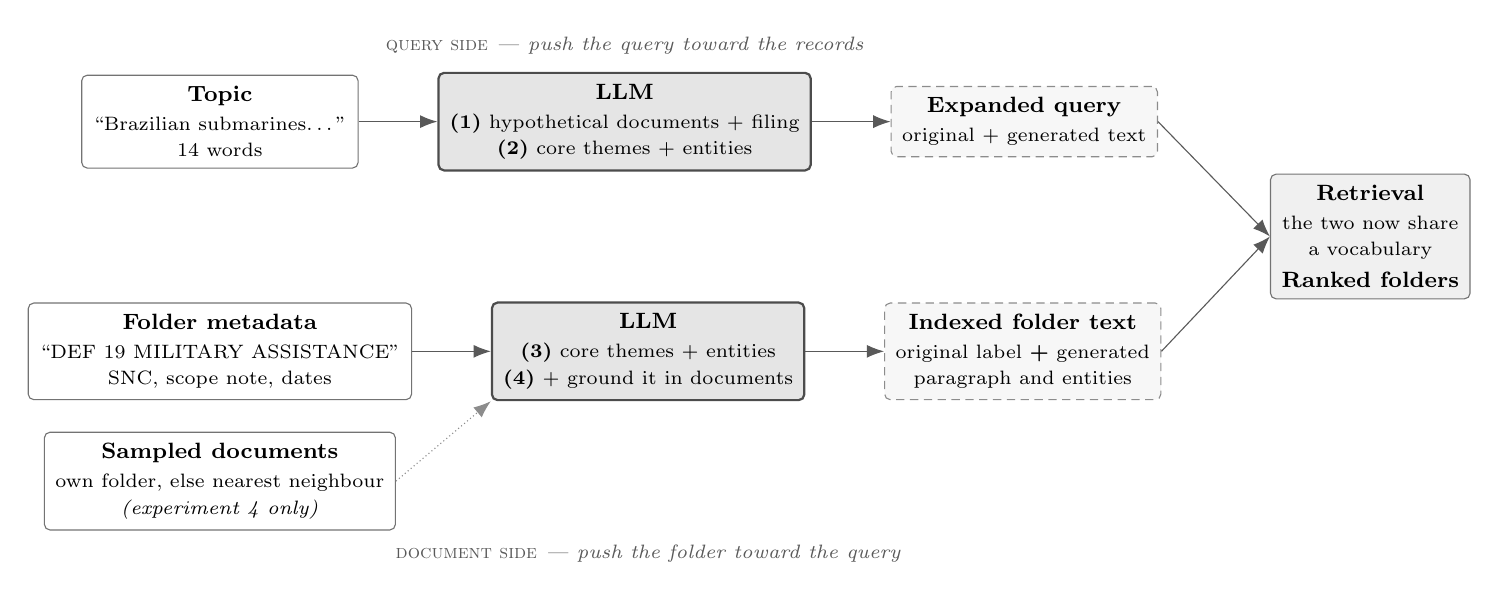
\begin{tikzpicture}[node distance=6mm]

% ---- query side ----
\node[dbox] (topic) {\textbf{Topic}\\[1pt]\scriptsize ``Brazilian submarines\ldots''\\\scriptsize 14 words};
\node[llmbox, right=10mm of topic] (qllm) {\textbf{LLM}\\[1pt]
  \scriptsize \textbf{(1)} hypothetical documents + filing\\
  \scriptsize \textbf{(2)} core themes + entities};
\node[outbox, right=10mm of qllm] (qexp) {\textbf{Expanded query}\\[1pt]
  \scriptsize original + generated text};

\draw[ar] (topic) -- (qllm);
\draw[ar] (qllm) -- (qexp);
\node[lbl, above=1mm of qllm] {\textsc{query side} --- push the query toward the records};

% ---- document side ----
\node[dbox, below=17mm of topic] (fold) {\textbf{Folder metadata}\\[1pt]
  \scriptsize ``DEF 19 MILITARY ASSISTANCE''\\\scriptsize SNC, scope note, dates};
\node[dbox, below=4mm of fold] (docs) {\textbf{Sampled documents}\\[1pt]
  \scriptsize own folder, else nearest neighbour\\\scriptsize \emph{(experiment 4 only)}};
\node[llmbox, right=10mm of fold] (dllm) {\textbf{LLM}\\[1pt]
  \scriptsize \textbf{(3)} core themes + entities\\
  \scriptsize \textbf{(4)} + ground it in documents};
\node[outbox, right=10mm of dllm] (daug) {\textbf{Indexed folder text}\\[1pt]
  \scriptsize original label \textbf{+} generated\\\scriptsize paragraph and entities};

\draw[ar] (fold) -- (dllm);
\draw[arw] (docs.east) -- (dllm.south west);
\draw[ar] (dllm) -- (daug);
\node[lbl, below=17mm of dllm] {\textsc{document side} --- push the folder toward the query};

% ---- they meet ----
\node[hit, anchor=west] (rank) at ($(qexp.east)!0.5!(daug.east) + (14mm,0)$) {\textbf{Retrieval}\\[1pt]
  \scriptsize the two now share\\\scriptsize a vocabulary\\[2pt]\textbf{Ranked folders}};
\draw[ar] (qexp.east) -- (rank.west);
\draw[ar] (daug.east) -- (rank.west);

\end{tikzpicture}}
\end{center}

\vspace{-2pt}

\begin{multicols}{2}

\textbf{The idea.} Using an LLM to rewrite both sides (queries and documents/folders metadata) into the same vocabulary:
three experiments expand the query toward the records or the folder toward the query, and a
fourth is running now. Each one below is: what it is, the prompt, real output, and what it
did to the numbers. The tables at the end put all of it in one grid.

\subsection*{What every prompt starts with}

Each of the prompts below opens with the same paragraph, so the model knows which archive it
is reasoning about before it is asked anything. It appears in the prompts as
\texttt{\{\{COLLECTION\_CONTEXT\}\}}:

{\scriptsize
\begin{verbatim}
COLLECTION CONTEXT:
These records were created by the U.S. Department of
State between 1963 and 1973 and maintained by the
Department, later transferred
to the U.S. National Archives. The period spans the
Goulart government, the March 1964 military coup, and
the military governments that followed (Castelo
Branco, Costa e Silva, Medici), including
Institutional Act No. 5 and the subsequent
intensification of censorship and repression. Folders
are labeled with Subject-Numeric Codes (SNC): a
three-letter primary subject (e.g., POL for Political
Affairs & Relations), a country code (almost always
BRAZ), and a numeric subdivision whose meaning is
specific to the primary subject.
\end{verbatim}
}

The period framing matters: it is what lets the model answer in 1960s State Department
vocabulary rather than in modern words.

\partrule

\section{HyDE: invent the documents the topic is asking for}

\textbf{What it is.} I ask the model to write what the answer documents and folder labels would look like to match the query. Two prompts per
topic. In the tables this is the \textbf{+HyDE} columns.


\begin{center}
\resizebox{\columnwidth}{!}{%
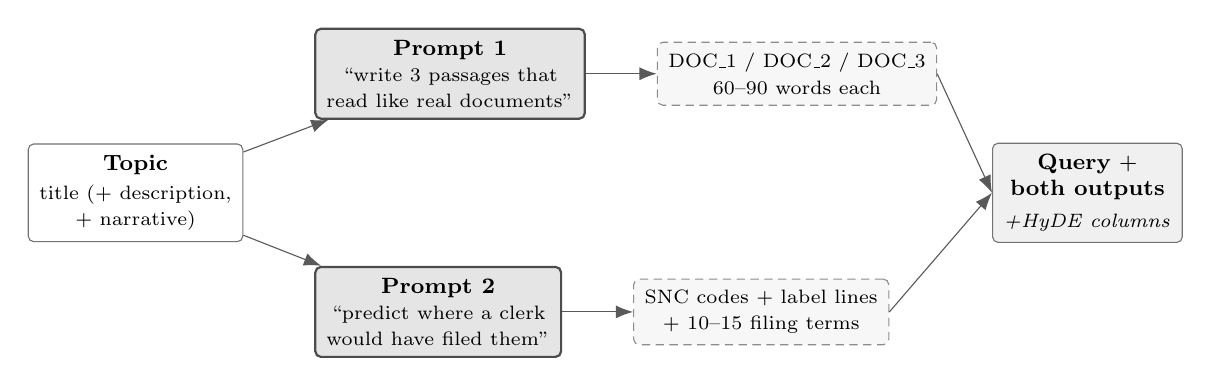
\begin{tikzpicture}[node distance=5mm]
\node[dbox] (q) {\textbf{Topic}\\[1pt]\scriptsize title (+ description,\\\scriptsize + narrative)};
\node[llmbox, above right=3mm and 9mm of q] (p1) {\textbf{Prompt 1}\\\scriptsize ``write 3 passages that\\\scriptsize read like real documents''};
\node[llmbox, below right=3mm and 9mm of q] (p2) {\textbf{Prompt 2}\\\scriptsize ``predict where a clerk\\\scriptsize would have filed them''};
\node[outbox, right=9mm of p1] (o1) {\scriptsize DOC\_1 / DOC\_2 / DOC\_3\\\scriptsize 60--90 words each};
\node[outbox, right=9mm of p2] (o2) {\scriptsize SNC codes + label lines\\\scriptsize + 10--15 filing terms};
\node[hit, anchor=west] (out) at ($(o1.east)!0.5!(o2.east) + (10mm,0)$) {\textbf{Query} +\\\textbf{both outputs}\\[2pt]\scriptsize \emph{+HyDE columns}};
\draw[ar] (q) -- (p1); \draw[ar] (q) -- (p2);
\draw[ar] (p1) -- (o1); \draw[ar] (p2) -- (o2);
\draw[ar] (o1.east) -- (out.west); \draw[ar] (o2.east) -- (out.west);
\end{tikzpicture}}
\end{center}

\subsection*{Prompt 1 --- hypothetical documents}

{\scriptsize
\begin{verbatim}
{{COLLECTION_CONTEXT}}

You are an expert historian of U.S.-Brazil relations
reconstructing the documentary record. A researcher is
looking for documents matching the information need
below. Write three short passages that read as if they
were excerpts from actual documents in this collection
that would satisfy this need.

INFORMATION NEED:
{{query_text}}

Write each passage as the document itself, not as a
description of it. Use the vocabulary, naming
conventions, abbreviations and phrasing of U.S. State
Department reporting from Brazil in the 1963-1973
period. Name the posts, officials, ministries,
agencies, programs, parties and places that such a
document would name. Do not hedge, do not use
conditional language, and do not refer to the
researcher or to the search. Start by "This document
is about..."

Do not invent specific telegram numbers, file
references or document identifiers.

Output exactly:

DOC_1: <60-90 words>
DOC_2: <60-90 words>
DOC_3: <60-90 words>

No other text.
\end{verbatim}
}

\subsection*{Output --- topic \emph{Brazilian submarines}}

The entire query: \emph{``Brazilian submarines / Find documents that mention the operation of
submarines by the Brazilian Navy.''}

\begin{quote}
\textbf{DOC\_1:} ``This document is about the Brazilian Navy's submarine operations. The
Embassy in Brasilia reports that the Brazilian Ministry of Navy has acquired two new
submarines from the UK. The submarines are expected to be operational by the end of 1965.
The Brazilian Navy's submarine fleet will be based in Rio de Janeiro.''

\textbf{DOC\_2:} ``\ldots a team of Brazilian Navy officers visited the US to discuss
submarine operations and maintenance. The team met with officials from the US Navy
Department and visited the submarine base in Norfolk, Virginia.''
\end{quote}

\subsection*{Prompt 2 --- where it would have been filed}

{\scriptsize
\begin{verbatim}
{{COLLECTION_CONTEXT}}

You are an expert archivist of the U.S. State
Department Subject-Numeric filing system. A researcher
is looking for documents matching the information need
below. Predict where in the filing system such
documents would have been filed.

INFORMATION NEED:
{{query_text}}

Records were filed at the time of creation
according to the administrative subject of the
document, not according to its later historical
interest. Choose codes on that basis: under what routine subject
heading would it have been filed.

Output exactly:

SNC_CODES: <3 to 5 codes, most likely first,
  comma-separated, in the form "POL 15-1">
LABEL_TEXT: <one line per code, in the form "<code>
  <expanded meaning of the code> BRAZ <year or year
  range>">
SUBJECT_TERMS: <10-15 terms, comma-separated, in the
  register of folder labels and filing headings:
  subject headings, office and agency names, country
  and place names. Not prose, not full sentences.>

No other text.
\end{verbatim}
}

\subsection*{Output --- same topic}

\begin{quote}
\textbf{SNC\_CODES:} DEF 6, POL 15-1, DEF 15

\textbf{LABEL\_TEXT:} ``DEF 6 Defense Affairs BRAZ 1963-1973'' / ``POL 15-1 Naval Forces BRAZ
1963-1973'' / ``DEF 15 Military Operations BRAZ 1963-1973''

\textbf{SUBJECT\_TERMS:} Brazilian Navy, Submarines, Naval Operations, Defense Affairs,
Maritime Defense, Naval Bases, Fleet Operations, Submarine Warfare, Anti-Submarine Warfare,
Naval Strategy\ldots
\end{quote}

It is guessing what folder labels are actually written in.

\partrule

\section{Core themes}

\textbf{What it is.} A different bet from HyDE: instead of inventing documents, restate the
need in period terminology and list the entities such documents would name. One prompt per
topic. In the tables this is the \textbf{+CT} columns.


\begin{center}
\resizebox{\columnwidth}{!}{%
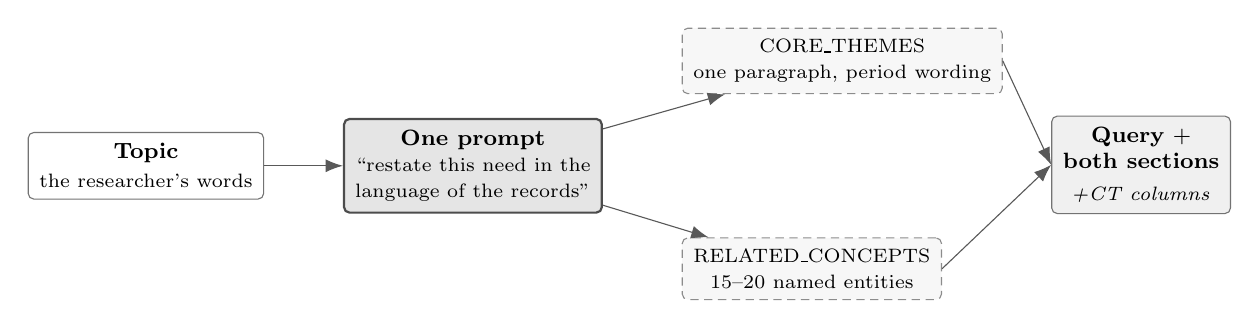
\begin{tikzpicture}[node distance=5mm]
\node[dbox] (q) {\textbf{Topic}\\[1pt]\scriptsize the researcher's words};
\node[llmbox, right=10mm of q] (p) {\textbf{One prompt}\\\scriptsize ``restate this need in the\\\scriptsize language of the records''};
\node[outbox, above right=3mm and 10mm of p] (o1) {\scriptsize CORE\_THEMES\\\scriptsize one paragraph, period wording};
\node[outbox, below right=3mm and 10mm of p] (o2) {\scriptsize RELATED\_CONCEPTS\\\scriptsize 15--20 named entities};
\node[hit, anchor=west] (out) at ($(o1.east)!0.5!(o2.east) + (10mm,0)$) {\textbf{Query} +\\\textbf{both sections}\\[2pt]\scriptsize \emph{+CT columns}};
\draw[ar] (q) -- (p);
\draw[ar] (p) -- (o1); \draw[ar] (p) -- (o2);
\draw[ar] (o1.east) -- (out.west); \draw[ar] (o2.east) -- (out.west);
\end{tikzpicture}}
\end{center}

\subsection*{Prompt}

{\scriptsize
\begin{verbatim}
{{COLLECTION_CONTEXT}}

You are an expert archivist and historian of
U.S.-Brazil relations helping a researcher search this
collection. Below is the researcher's information
need.

INFORMATION NEED:
{{query_text}}

Output exactly two labeled sections and nothing else.
No preamble, no markdown, no commentary.

CORE_THEMES: <one paragraph, 80-120 words>
RELATED_CONCEPTS: <comma-separated list of 15-20
terms>

CORE_THEMES must restate this information need as it
would be expressed in the language of the records
themselves: State Department terminology of the
1963-1973 period, naming the institutions, actors,
policies and events that documents satisfying this
need would discuss. Write it as a description of the
documents being sought, not as a question or a
request.

RELATED_CONCEPTS must list specific historical
entities, institutions, programs, treaties, places,
technologies and diplomatic terms that such documents
would name. Include Portuguese terms where they are
the form actually used in the period. Do not include
generic words and do not include terms unrelated to
this information need.
\end{verbatim}
}

\subsection*{Output --- same topic}

\begin{quote}
\textbf{CORE\_THEMES:} ``Documents pertaining to the Brazilian Navy's submarine operations,
including those related to the Marinha do Brasil's acquisition, maintenance, and deployment
of submarines, as well as U.S.\ diplomatic efforts to cooperate with or influence Brazil's
naval modernization programs, particularly during the Goulart and subsequent military
governments.''

\textbf{RELATED\_CONCEPTS:} Marinha do Brasil, naval modernization, Goulart government,
Castelo Branco, Costa e Silva, Medici, Institutional Act No.~5, U.S.\ Military Assistance
Program, Foreign Military Sales, Rio Treaty, For\c{c}a de Submarinos, Base Naval de Aratu,
Estado-Maior da Marinha\ldots (27 terms)
\end{quote}

\partrule

\section{Folder augmentation}

\textbf{What it is.} The other side of the match. For all 1{,}336 folders, the model writes what records filed under that classification
would concern, and that text is appended to the folder's own label in the index. In the tables
this is the
\textbf{FL-aug} columns.


\begin{center}
\resizebox{\columnwidth}{!}{%
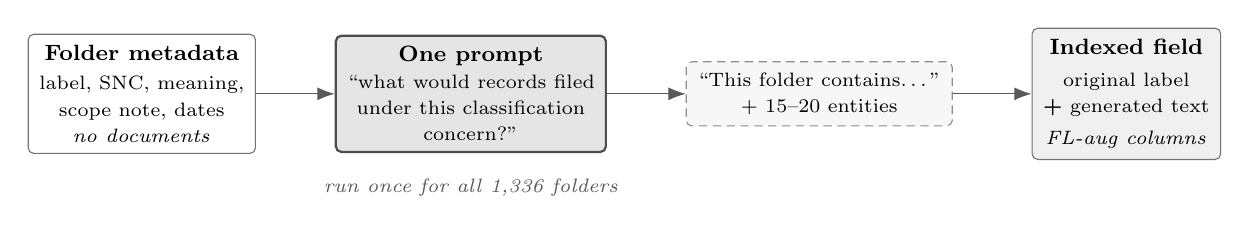
\begin{tikzpicture}[node distance=5mm]
\node[dbox] (m) {\textbf{Folder metadata}\\[1pt]\scriptsize label, SNC, meaning,\\\scriptsize scope note, dates\\\scriptsize \emph{no documents}};
\node[llmbox, right=10mm of m] (p) {\textbf{One prompt}\\\scriptsize ``what would records filed\\\scriptsize under this classification\\\scriptsize concern?''};
\node[outbox, right=10mm of p] (o) {\scriptsize ``This folder contains\ldots''\\\scriptsize + 15--20 entities};
\node[hit, right=10mm of o] (idx) {\textbf{Indexed field}\\[2pt]\scriptsize original label\\\scriptsize \textbf{+} generated text\\[2pt]\scriptsize \emph{FL-aug columns}};
\draw[ar] (m) -- (p); \draw[ar] (p) -- (o); \draw[ar] (o) -- (idx);
\node[lbl, below=2mm of p] {run once for all 1{,}336 folders};
\end{tikzpicture}}
\end{center}

\subsection*{Prompt}

{\scriptsize
\begin{verbatim}
{{COLLECTION_CONTEXT}}

You are an expert archivist and historian of
U.S.-Brazil relations. Below is the archival
classification of one physical folder. No documents
from this folder are available. Your task is to
describe what records filed under this classification,
in this collection and this period, would concern - so
that a researcher's query can be matched against this
folder even though its contents have not been
digitized.

CLASSIFICATION:
- Folder Label: {{folder_label}}
- Subject-Numeric Code: {{snc}}
- Meaning: {{parent_expanded_snc}}
- Scope Note: {{scope_note}}
- Date Range: {{start_date}} to {{end_date}}

Output exactly two labeled sections and nothing else.
No preamble, no markdown, no commentary.

CORE_THEMES: <one paragraph, 100-150 words>
RELATED_CONCEPTS: <comma-separated list of 15-20
terms>

CORE_THEMES must begin with "This folder contains" and
describe the thematic scope implied by the
classification, situated in Brazil in the years given
by the date range. Draw on established historical
knowledge of that subject in that period: the
institutions, actors, policies and events that records
of this kind would concern. Do NOT invent specific
documents, specific telegram numbers, or specific
incidents you cannot ground in the classification and
the historical record.

RELATED_CONCEPTS must list specific historical
entities, institutions, programs, treaties, places,
technologies and diplomatic terms that records under
this classification, in this period, would plausibly
name. Include Portuguese terms where they are the form
actually used in the period.
\end{verbatim}
}

\subsection*{Output --- one real folder}

Everything the catalogue holds about it: label \texttt{DEF 19 MILITARY ASSISTANCE}, meaning
\textsc{defense affairs: military assistance}, no scope note, dates unknown.

\begin{quote}
\textbf{CORE\_THEMES:} ``This folder contains records related to military assistance provided
by the United States to Brazil during a period of significant political upheaval, including
the Goulart government, the 1964 military coup, and the subsequent military regimes. The
documents would likely concern the negotiation, implementation, and evaluation of military
aid programs, including the provision of equipment, training, and personnel. The records may
also touch on the role of Brazilian military institutions, such as the Ex\'ercito Brasileiro,
Marinha do Brasil, and For\c{c}a A\'erea Brasileira\ldots''

\textbf{RELATED\_CONCEPTS:} U.S.\ Military Assistance Program, Ex\'ercito Brasileiro, Marinha
do Brasil, For\c{c}a A\'erea Brasileira, National Security Doctrine, Brazilian Ministry of
War, Military Assistance Advisory Group, Escola Superior de Guerra, Acordo de Assist\^encia
Militar, Rio Treaty\ldots (27 terms)
\end{quote}

The indexed field becomes the original label \emph{plus} that paragraph and its 27 entities, so
a query about the Brazilian Navy
finally has something to match in a folder nobody has scanned. That is also the risk: nothing
in this folder's metadata guarantees the Marinha do Brasil is really in it.

\partrule

\section{Running now: ground the description in real documents}

\textbf{What it is.} Everything above was written from the classification alone. But a folder
often \emph{does} have a few digitized documents in the sample --- and when it doesn't, its
neighbours do. This experiment shows the model that evidence and asks it to merge
classification and documents into one description.

\begin{itemize}
\item Evidence comes in strict order, first non-empty source wins, never mixed: the folder's
      own sampled documents $\rightarrow$ same SNC $\rightarrow$ similar SNC $\rightarrow$ same
      box. Capped at 5 documents.
\item \textbf{So the augmentation becomes per seed:} the sample changes with the seed, so each
      of the 30 seeds gets its own 1{,}336 descriptions rather than one set shared by all runs.
      I record which of the four sources each description used, so results can be split by how
      well-evidenced the folders were.
\end{itemize}


\begin{center}
\resizebox{\columnwidth}{!}{%
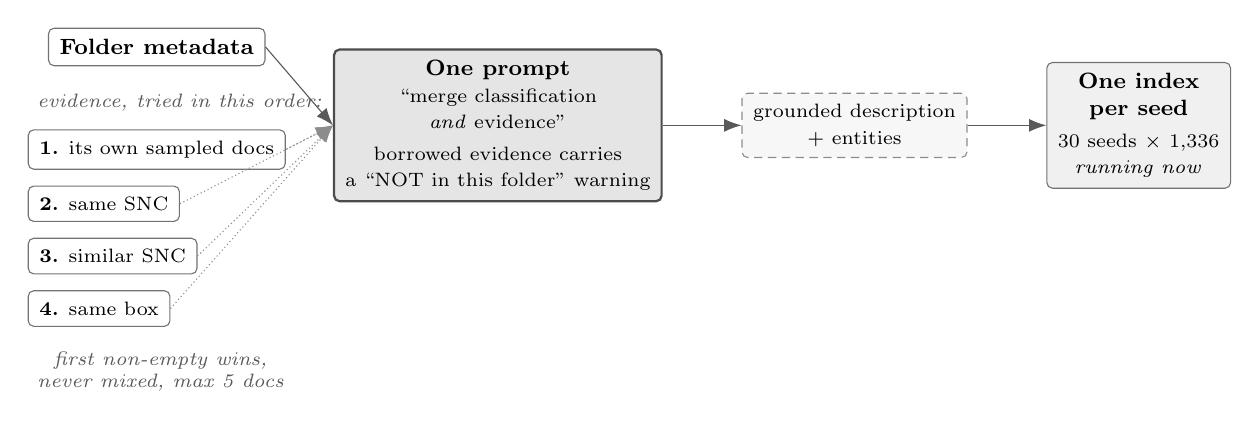
\begin{tikzpicture}[node distance=5mm]
\node[dbox] (m) {\textbf{Folder metadata}};
\node[dbox, below=8mm of m] (e1) {\scriptsize \textbf{1.} its own sampled docs};
\node[dbox, anchor=north west] (e2) at ($(e1.south west) + (0,-2mm)$) {\scriptsize \textbf{2.} same SNC};
\node[dbox, anchor=north west] (e3) at ($(e2.south west) + (0,-2mm)$) {\scriptsize \textbf{3.} similar SNC};
\node[dbox, anchor=north west] (e4) at ($(e3.south west) + (0,-2mm)$) {\scriptsize \textbf{4.} same box};
\node[lbl, anchor=north west] (fb) at ($(e4.south west) + (0,-2mm)$) {first non-empty wins,\\never mixed, max 5 docs};
\node[lbl, anchor=south west] at ($(e1.north west) + (0,1mm)$) {evidence, tried in this order:};
\node[llmbox, anchor=west] (p) at ($(m.east)!0.5!(e2.east) + (14mm,0)$) {\textbf{One prompt}\\\scriptsize ``merge classification\\\scriptsize \emph{and} evidence''\\[2pt]\scriptsize borrowed evidence carries\\\scriptsize a ``NOT in this folder'' warning};
\node[outbox, right=10mm of p] (o) {\scriptsize grounded description\\\scriptsize + entities};
\node[hit, right=10mm of o] (idx) {\textbf{One index}\\\textbf{per seed}\\[2pt]\scriptsize 30 seeds $\times$ 1{,}336\\\scriptsize \emph{running now}};
\draw[ar] (m.east) -- (p.west);
\draw[arw] (e1.east) -- (p.west); \draw[arw] (e2.east) -- (p.west);
\draw[arw] (e3.east) -- (p.west); \draw[arw] (e4.east) -- (p.west);
\draw[ar] (p) -- (o); \draw[ar] (o) -- (idx);
\end{tikzpicture}}
\end{center}

\subsection*{Prompt}

{\scriptsize
\begin{verbatim}
{{COLLECTION_CONTEXT}}

You are an expert archivist and historian of
U.S.-Brazil relations. Below is the archival
classification of one physical folder, together with
document evidence. Merge them into a single
folder-level description that will be indexed for
retrieval.

CLASSIFICATION:
- Folder Label: {{folder_label}}
- Subject-Numeric Code: {{snc}}
- Meaning: {{parent_expanded_snc}}
- Scope Note: {{scope_note}}
- Date Range: {{start_date}} to {{end_date}}

{{EVIDENCE_BLOCK}}

Output exactly two labeled sections and nothing else.
No preamble, no markdown, no commentary.

CORE_THEMES: <one paragraph, 100-150 words>
RELATED_CONCEPTS: <comma-separated list of 15-20
terms>

CORE_THEMES must begin with "This folder contains" and
combine the classification's scope with the concrete
evidence above, in State Department terminology of the
era. Draw on established historical knowledge to make
explicit the geopolitical context, institutions and
policies implicit in this material, so that queries
which do not use the folder's exact wording can still
match it. Do not invent specific incidents, telegram
numbers or named individuals that neither the evidence
nor the historical record supports.

RELATED_CONCEPTS must list specific entities,
institutions, programs, treaties, places and
diplomatic terms that are either present in the
evidence or historically bound to this subject and
period. Include Portuguese terms where they are the
form actually used.
\end{verbatim}
}

\subsection*{The evidence block, two versions}

When the documents really are the folder's own, it is just a list:

{\scriptsize
\begin{verbatim}
DOCUMENTS IN THIS FOLDER:
- <title> - <summary>
- ...
\end{verbatim}
}

When they are borrowed from a neighbour, the block warns the model explicitly --- the whole
risk being that it attributes a neighbour's contents to this folder:

{\scriptsize
\begin{verbatim}
DOCUMENTS FROM RELATED FOLDERS (CONTEXTUAL EVIDENCE
ONLY):
The following documents are NOT in this folder. They
come from folders that are nearby in the archive or
share this folder's classification, and are shown only
to indicate the kind of material this part of the
collection holds. Do not state or imply that these
specific documents, incidents or communications are in
this folder.
- [from folder with same snc relation]: <title> -
  <summary>
- ...
\end{verbatim}
}

\textbf{What it should tell us.} Compared against the \emph{FL-aug} columns, everything else
fixed: does grounding in real sampled text beat describing a folder from its classification
--- and does the gain survive when the evidence had to be borrowed from a neighbour? No
results yet; generation is in progress.

\partrule

\section{All of it in one grid}

The tables overleaf cross the three finished experiments. Reading the columns:

\begin{itemize}
\item \textbf{Plain folder label} --- document side untouched; \emph{Base} is the no-LLM
      baseline.
\item \textbf{FL-aug: ALLFL partner} --- only the folder-level ranker's labels augmented.
\item \textbf{FL-aug: doc.\ field} --- the main ranker's folder-label field augmented too;
      the most LLM text in play.
\item \textbf{+HyDE} / \textbf{+CT} --- the two query expansions, never combined.
\end{itemize}

Bold marks the largest number in a row and nothing more: no significance testing was applied.

\end{multicols}

\clearpage

% Generated by src/stats_test/build_results_tables.py -- do not edit by hand.
% Re-run after adding runs to all_runs/ to refresh.

\begin{table*} [t]
\centering
\caption{nDCG@5, Title (T{-}{-}) queries, uniform sampling (U5, 30-seed random protocol). Columns escalate the amount of folder-label augmentation applied to the document side: \textbf{FL-aug: ALLFL partner} augments only the separate all-folders-label ranker's labels; \textbf{FL-aug: doc.\ field} augments the main ranker's own \texttt{folderlabel} field (and, for the hybrid rows, the partner as well). \textbf{+HyDE} expands the query with hypothetical documents and a hypothetical folder label; \textbf{+CT} expands it with the topic's core themes and related concepts --- these are two different expansions. Bold marks the highest value in each row; no significance testing is applied, so bold indicates only the larger number and not a demonstrated difference. \texttt{---} marks a cell with no run behind it, either because the configuration does not exist for that row (the partner columns for non-hybrid rows, the doc.\ field columns for the pure-ALLFL rows) or because it has not been generated yet.}
\label{tab:fl-T}
\resizebox{\textwidth}{!}{
\begin{tabular}{| l || c | c || c | c || c | c | c |}
\hline
\multicolumn{1}{|c||}{} &
\multicolumn{2}{c||}{\textbf{Plain folder label}} &
\multicolumn{2}{c||}{\textbf{FL-aug: ALLFL partner}} &
\multicolumn{3}{c|}{\textbf{FL-aug: doc.\ field}} \\
\hline
\textbf{Configuration} & \textbf{Base} & \textbf{+HyDE} & \textbf{Base} & \textbf{+CT} & \textbf{Base} & \textbf{+HyDE} & \textbf{+CT} \\
\hline
\texttt{B.{-}{-}F{-}.{-}.{-}} & 0.0525 & 0.1178 & --- & --- & 0.0877 & --- & \textbf{0.1385} \\
\hline
\texttt{B.TOFS.{-}.{-}} & 0.1801 & 0.2293 & --- & --- & 0.1853 & \textbf{0.2333} & 0.1647 \\
\texttt{L.TOFS.mx{-}{-}2.{-}} & 0.1849 & \textbf{0.2335} & --- & --- & 0.1853 & 0.2282 & 0.1587 \\
\texttt{C.TOFS.{-}.{-}} & \textbf{0.1833} & 0.1519 & --- & --- & 0.1774 & 0.1494 & 0.1436 \\
\texttt{E.TOFS.{-}.{-}} & \textbf{0.2195} & 0.1978 & --- & --- & 0.2173 & 0.2058 & 0.2074 \\
\texttt{Z.TOFS.{-}.{-}} & 0.2133 & 0.2277 & --- & --- & 0.2152 & \textbf{0.2366} & 0.2044 \\
\texttt{W.TOFS.{-}.{-}} & 0.2167 & 0.2299 & --- & --- & 0.2167 & \textbf{0.2353} & 0.2021 \\
\hline
\texttt{V.TOFS.mx{-}{-}2.b} & 0.2158 & 0.2532 & 0.2338 & 0.2603 & 0.2299 & \textbf{0.2756} & 0.2154 \\
\texttt{X.TOFS.mx{-}{-}2.b} & 0.2101 & 0.2519 & 0.2335 & 0.2561 & 0.2332 & \textbf{0.2807} & 0.2196 \\
\texttt{W.TOFS.{-}.c} & 0.2347 & 0.2081 & 0.2584 & 0.2547 & 0.2590 & \textbf{0.2770} & 0.2330 \\
\texttt{W.TOFS.s{-}{-}{-}2.c} & 0.2390 & 0.2134 & 0.2651 & 0.2643 & 0.2637 & \textbf{0.2839} & 0.2423 \\
\hline
\texttt{{-}.{-}{-}{-}{-}.{-}.b} & 0.0907 & 0.1453 & 0.1690 & \textbf{0.2182} & --- & --- & --- \\
\texttt{{-}.{-}{-}{-}{-}.{-}.c} & 0.1347 & 0.0327 & \textbf{0.1774} & 0.1733 & --- & --- & --- \\
\texttt{{-}.{-}{-}{-}{-}.{-}.e} & 0.1467 & 0.1371 & 0.2164 & \textbf{0.2560} & --- & --- & --- \\
\hline
\end{tabular}
}
% TODO: missing cells above -- FL-aug doc. field x +HyDE: python -m src.llm_experiments.runs.run_table_completion_experiments FLDOC
\end{table*}

\begin{table*} [t]
\centering
\caption{nDCG@5, Title+Desc (TD-) queries, uniform sampling (U5, 30-seed random protocol). Columns escalate the amount of folder-label augmentation applied to the document side: \textbf{FL-aug: ALLFL partner} augments only the separate all-folders-label ranker's labels; \textbf{FL-aug: doc.\ field} augments the main ranker's own \texttt{folderlabel} field (and, for the hybrid rows, the partner as well). \textbf{+HyDE} expands the query with hypothetical documents and a hypothetical folder label; \textbf{+CT} expands it with the topic's core themes and related concepts --- these are two different expansions. Bold marks the highest value in each row; no significance testing is applied, so bold indicates only the larger number and not a demonstrated difference. \texttt{---} marks a cell with no run behind it, either because the configuration does not exist for that row (the partner columns for non-hybrid rows, the doc.\ field columns for the pure-ALLFL rows) or because it has not been generated yet.}
\label{tab:fl-TD}
\resizebox{\textwidth}{!}{
\begin{tabular}{| l || c | c || c | c || c | c | c |}
\hline
\multicolumn{1}{|c||}{} &
\multicolumn{2}{c||}{\textbf{Plain folder label}} &
\multicolumn{2}{c||}{\textbf{FL-aug: ALLFL partner}} &
\multicolumn{3}{c|}{\textbf{FL-aug: doc.\ field}} \\
\hline
\textbf{Configuration} & \textbf{Base} & \textbf{+HyDE} & \textbf{Base} & \textbf{+CT} & \textbf{Base} & \textbf{+HyDE} & \textbf{+CT} \\
\hline
\texttt{B.{-}{-}F{-}.{-}.{-}} & 0.0488 & 0.1000 & --- & --- & 0.0794 & --- & \textbf{0.1406} \\
\hline
\texttt{B.TOFS.{-}.{-}} & 0.1810 & \textbf{0.2294} & --- & --- & 0.1728 & 0.2285 & 0.2057 \\
\texttt{L.TOFS.mx{-}{-}2.{-}} & 0.1852 & \textbf{0.2364} & --- & --- & 0.1738 & 0.2205 & 0.1914 \\
\texttt{C.TOFS.{-}.{-}} & \textbf{0.1734} & 0.1626 & --- & --- & 0.1660 & 0.1553 & 0.1527 \\
\texttt{E.TOFS.{-}.{-}} & 0.1802 & 0.1836 & --- & --- & 0.1941 & \textbf{0.1977} & 0.1926 \\
\texttt{Z.TOFS.{-}.{-}} & 0.1987 & 0.2250 & --- & --- & 0.2055 & \textbf{0.2316} & 0.2220 \\
\texttt{W.TOFS.{-}.{-}} & 0.2044 & 0.2273 & --- & --- & 0.2067 & \textbf{0.2296} & 0.2185 \\
\hline
\texttt{V.TOFS.mx{-}{-}2.b} & 0.2127 & 0.2499 & 0.2426 & \textbf{0.2937} & 0.2289 & 0.2606 & 0.2598 \\
\texttt{X.TOFS.mx{-}{-}2.b} & 0.2074 & 0.2470 & 0.2365 & \textbf{0.2897} & 0.2263 & 0.2640 & 0.2654 \\
\texttt{W.TOFS.{-}.c} & 0.2132 & 0.2186 & 0.2569 & \textbf{0.2764} & 0.2525 & 0.2756 & 0.2571 \\
\texttt{W.TOFS.s{-}{-}{-}2.c} & 0.2144 & 0.2229 & 0.2647 & \textbf{0.2857} & 0.2607 & 0.2850 & 0.2681 \\
\hline
\texttt{{-}.{-}{-}{-}{-}.{-}.b} & 0.0972 & 0.1390 & 0.1671 & \textbf{0.2384} & --- & --- & --- \\
\texttt{{-}.{-}{-}{-}{-}.{-}.c} & 0.0940 & 0.0586 & 0.1933 & \textbf{0.2019} & --- & --- & --- \\
\texttt{{-}.{-}{-}{-}{-}.{-}.e} & 0.0880 & 0.1085 & \textbf{0.2408} & 0.2206 & --- & --- & --- \\
\hline
\end{tabular}
}
% TODO: missing cells above -- FL-aug doc. field x +HyDE: python -m src.llm_experiments.runs.run_table_completion_experiments FLDOC
\end{table*}

\begin{table*} [t]
\centering
\caption{nDCG@5, Title+Desc+Narr (TDN) queries, uniform sampling (U5, 30-seed random protocol). Columns escalate the amount of folder-label augmentation applied to the document side: \textbf{FL-aug: ALLFL partner} augments only the separate all-folders-label ranker's labels; \textbf{FL-aug: doc.\ field} augments the main ranker's own \texttt{folderlabel} field (and, for the hybrid rows, the partner as well). \textbf{+HyDE} expands the query with hypothetical documents and a hypothetical folder label; \textbf{+CT} expands it with the topic's core themes and related concepts --- these are two different expansions. Bold marks the highest value in each row; no significance testing is applied, so bold indicates only the larger number and not a demonstrated difference. \texttt{---} marks a cell with no run behind it, either because the configuration does not exist for that row (the partner columns for non-hybrid rows, the doc.\ field columns for the pure-ALLFL rows) or because it has not been generated yet.}
\label{tab:fl-TDN}
\resizebox{\textwidth}{!}{
\begin{tabular}{| l || c | c || c | c || c | c | c |}
\hline
\multicolumn{1}{|c||}{} &
\multicolumn{2}{c||}{\textbf{Plain folder label}} &
\multicolumn{2}{c||}{\textbf{FL-aug: ALLFL partner}} &
\multicolumn{3}{c|}{\textbf{FL-aug: doc.\ field}} \\
\hline
\textbf{Configuration} & \textbf{Base} & \textbf{+HyDE} & \textbf{Base} & \textbf{+CT} & \textbf{Base} & \textbf{+HyDE} & \textbf{+CT} \\
\hline
\texttt{B.{-}{-}F{-}.{-}.{-}} & 0.0716 & 0.1219 & --- & --- & 0.1041 & --- & \textbf{0.1250} \\
\hline
\texttt{B.TOFS.{-}.{-}} & 0.1991 & \textbf{0.2331} & --- & --- & 0.2020 & 0.2238 & 0.2175 \\
\texttt{L.TOFS.mx{-}{-}2.{-}} & 0.2071 & \textbf{0.2403} & --- & --- & 0.2001 & 0.2175 & 0.2072 \\
\texttt{C.TOFS.{-}.{-}} & \textbf{0.1679} & 0.1655 & --- & --- & 0.1622 & 0.1622 & 0.1622 \\
\texttt{E.TOFS.{-}.{-}} & 0.1927 & 0.1940 & --- & --- & \textbf{0.2030} & 0.2005 & 0.1949 \\
\texttt{Z.TOFS.{-}.{-}} & 0.2114 & 0.2289 & --- & --- & 0.2232 & \textbf{0.2323} & 0.2287 \\
\texttt{W.TOFS.{-}.{-}} & 0.2156 & \textbf{0.2361} & --- & --- & 0.2227 & 0.2276 & 0.2258 \\
\hline
\texttt{V.TOFS.mx{-}{-}2.b} & 0.2163 & 0.2536 & 0.2533 & \textbf{0.2832} & 0.2464 & 0.2526 & 0.2605 \\
\texttt{X.TOFS.mx{-}{-}2.b} & 0.2113 & 0.2477 & 0.2486 & \textbf{0.2807} & 0.2458 & 0.2582 & 0.2641 \\
\texttt{W.TOFS.{-}.c} & 0.2226 & 0.2326 & 0.2690 & \textbf{0.2804} & 0.2662 & 0.2679 & 0.2648 \\
\texttt{W.TOFS.s{-}{-}{-}2.c} & 0.2302 & 0.2366 & 0.2758 & \textbf{0.2866} & 0.2762 & 0.2787 & 0.2753 \\
\hline
\texttt{{-}.{-}{-}{-}{-}.{-}.b} & 0.1079 & 0.1463 & 0.1845 & \textbf{0.2155} & --- & --- & --- \\
\texttt{{-}.{-}{-}{-}{-}.{-}.c} & 0.0949 & 0.0775 & \textbf{0.1980} & 0.1980 & --- & --- & --- \\
\texttt{{-}.{-}{-}{-}{-}.{-}.e} & 0.1284 & 0.1178 & 0.2564 & \textbf{0.2687} & --- & --- & --- \\
\hline
\end{tabular}
}
% TODO: missing cells above -- FL-aug doc. field x +HyDE: python -m src.llm_experiments.runs.run_table_completion_experiments FLDOC
\end{table*}

\end{document}
